
\Chapter{
}{The roles and physics of aeolian dust}\label{chap:dust_roles_models}
Aeolian dust is one of the most abundant aerosol species in the atmosphere and accounts for most of the total atmospheric aerosol mass \parencite{adebiyi2020dust}.
Aeolian dust refers to dust that is emitted and transport
ted by winds and the word aeolian stems from the Greek god Aeolus, which in Greek mythology is the keeper of the winds. 
Around 1/3 of the earth surface is covered by deserts, that is, regions where the precipitation is too low and evaporation too high to allow plants to grow \parencite{williams_climate_2014}.
As shown in \Cref{fig:desert_distrubtion} a large portion of the arid regions are located between 20\degree - 40\degree north/south. 
This region is known as the dust belt\parencite{williams_climate_2014}. 
The dust belt coincides with the descending part of the Hadley circulation, where the descending motion increases the atmosphere's stability and suppress the formation of rainfall, e.g., Sahara desert. 
Other areas that typically experience a minimal amount of rainfall are places situated in the rain shadow of the surrounding topography (e.g. Atacama desert) or far in the interior of the continents where there are no proximal sources of moisture (e.g. Gobi desert).  
% The main aeolian dust sources are found in regions such as the Sahara, Middle East and northwest China.
The dry conditions produce loose soils that are easily erodible. 
Thus during periods of strong winds, dust emissions are naturally produced and entrained into the atmosphere. 
The world's deserts produce an estimated 2000Mt of atmospheric dust globally each year, with around 1500Mt being deposited on land and about 500Mt being deposited into the ocean \parencite{shao2011dust}. 

This chapter aims to examine the different roles of aeolian dust in the climate system, how dust deposits can serve as a valuable record of environmental change, and to describe the physical processes that go into current dust models. In order to give context and motivation to why we study and model dust and to provide prerequisite knowledge to inform the interpretation of the results and discussion in \Cref{Chap:Results} and \Cref{chap:Discussion}.  

\begin{figure}[htpb]
    \centering
    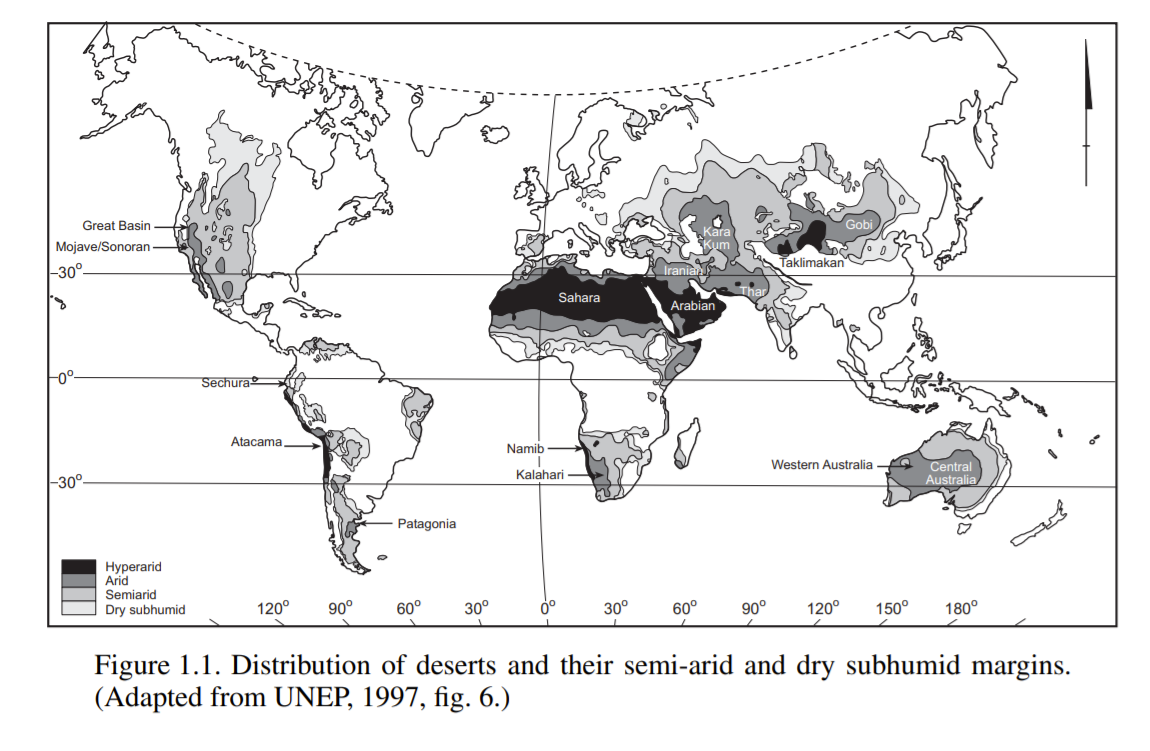
\includegraphics[width=\textwidth]{texfiles/figs/Desert_distrubtion.PNG}
    \caption{Earth's distribution of arid regions, adopted from \textcite{williams_climate_2014}}
    \label{fig:desert_distrubtion}
\end{figure}

\section{Dust's role in the climate system}\label{seq:physics_of_dust}
\subsection{Climate feedback of dust}
 
In the atmosphere, the dust particles directly affect the transfer of radiation through the atmosphere. 
The smallest dust particles between 0.2-\SI{2}{\micro\metre} have a size around the same order as the wavelength of visible light and are the most efficient at scattering incoming solar radiation back to space. 
Accordingly, the smallest particles have a cooling effect on climate. 
Conversely, the larger particles (> \SI{4}{\micro\metre}) produces has a warming effect on climate due to their larger size, which makes them efficient at absorbing terrestrial longwave radiation \parencite{choobari2014global}.
The lifetime of the dust aerosols is also strongly dependent on particle size \parencite{mahowald2014size}. Dust that gets entrained into the upper troposphere can be transported by the winds for thousands of kilometres and stay in the atmosphere for a long time \parencite{yumimoto_elevated_2009}. Constraining the direct radiative effect of dust aerosols thus requires getting both the magnitude and the size distribution of the emitted dust correct \parencite{adebiyi2020dust}.

Dust aerosol also interacts with clouds by acting as \acrfull{in} and \acrfull{ccn} altering the microphysical properties of the clouds \parencite{lohmann2006sensitivity}. 
Dust aerosols in their unaltered state are usually hydrophobic and thus quite inefficient \acrshort{ccn}. 
However, during transport, dust aerosols can acquire a coating of soluble material, enhancing their ability to act as \acrshort{ccn} \parencite{Dust_aerosols_coating2001}. 
Dust aerosols have also been suggested to warm the clouds as dusty clouds have been observed to have a lower liquid water path compared to their dust-free counterparts \parencite{huang2006satellite}. 
The warming of the cloud induced by the dust aerosols might play a role in inhibiting precipitation over the desert regions, reinforcing the aridity of the desert \parencite{shao2011dust}.  However, there are large uncertainties in the radiative impact of dust aerosols on clouds due to how sensitive clouds' radiative effects are to even small changes in their microphysical properties (e.g. droplet size, droplet concentration and cloud phase).

Beyond the time dust reside in the atmosphere, dust deposition also has a large impact on climate through influencing ecosystems and changing the snow surface albedo \parencite{mahowald2010observed,shao2011dust,wittmann2017impact}. 
In particular, ocean biomass productivity is dependent on dust as a source of iron. Iron is a limiting factor for phytoplankton production, which is responsible for nearly half of the annual \ch{CO2} exchange between the atmosphere and the ocean and the majority of carbon sequestration \parencite{shao2011dust}. Moreover, African dust has been found to be an important source of nutrients for the Amazon rainforest. \textcite{yu2015fertilizing} estimated about 0.022 Tg of phosphorus is brought to the Amazon through deposition of Sharan dust each year, comparable to the amount washed out by rainfall. Model estimates have shown that the increased dust deposition to the ocean and the corresponding boost of ocean productivity during the 20th century has caused an additional 4ppm of \ch{CO2} to be taken up by the ocean. However, regional shifts in precipitation and temperature due to changes in dust aerosol caused a decrease of 6ppm \ch{CO2} in the terrestrial biosphere carbon sink \parencite{mahowald2010observed}. This highlights the uncertainty of the net influence of dust on the biosphere and the carbon cycle.
% There is no mentioning of the how dust affect snow surface albedo here????

\subsection{Dust as a climate archive}
Dust emission fluxes, size distribution and mineralogical composition are all strongly influenced by the wind speed, soil moisture and vegetation cover, and therefore indirectly modulating the influence of dust in the climate system. 
These climatic variables have experienced large changes throughout the history of Earth's climate and, more pressingly, are expected to change under the ongoing human-caused global warming. Dust transport is affected by changes in the atmospheric circulation and wet deposition by precipitation changes. 
There is, consequently, a potential for feedbacks involving dust and climate change.

Thus dust archives are a window into the past from which the interconnections between climate and dust can be studied and provide insight on how the impact of dust might change in the near future climate. 

Arguably the most important dust record is the Loess record. Loess consists of aeolian sediments and is typically heavily sorted dominated by silt-sized (2-\SI{50}{\micro\metre}) particles \parencite{muhs2014loess}. Terrestrial loess occupies large areas of North America, China, Central Asia and Europe, with the most prominent Loess deposits located at the \acrfull{clp}.
Variations in the \acrfull{mar} and particle size distribution have been used to reconstruct changes in large scale-circulation patterns and dust transport pathways \parencite{maher2016palaeoclimatic,ding2000re}, climatic changes in the dust source and deposition areas \parencite{shang2016variations,sun2005late}, and to provide constraints for model reconstructions of past global climate states \parencite{da2015early}. 
In addition to loess, aeolian dust is also found in ice cores and deep-sea records. One of the best-documented features in the dust record is the variation in \acrfull{mar} between the glacial and interglacial periods. 
During glacial stages, the earth experienced increased dust loading. Findings from the dust records suggest that during the glacial periods, the high latitude dust loading were up to 25 times the present value and around two times at the lower latitude \parencite{shao2011dust}.     


\section{Dust modelling}\label{sec:dust_modelling}
The important role of dust in the climate system, as pointed out in the previous section, has inspired researchers across the scientific disciplines to put considerable efforts towards developing global and regional dust models. 
The field of dust modelling started to take off in the early 1990s when scientists realised that aerosols, including dust, were responsible for a large fraction of the uncertainties in the climate models due to the difficulties in determining the aerosol radiative effect \parencite{tegen1996influence}, as described in \Cref{seq:physics_of_dust}. 
Models have improved since then, and current state of the art models can reproduce large scale patterns of atmospheric dust load \parencite{huneeus2011global}. 
However, uncertainties in the description of source areas and processes controlling dust emission and deposition produce a large spread in simulated dust fluxes \parencite{huneeus2011global}. 
This section provides an overview of the parameterisations of the full dust cycle, i.e., dust emissions, transport and deposition processes used in current dust models. 
%The last part of this chapter will discuss some of the main discrepancies and uncertainties of current dust models.
 
\subsection{Dust emissions}\label{sec:dust_emission_modelling}
Producing a realistic estimate of the spatial distribution of dust emission flux depends on the model having a realistic representation of both the land surface properties and surface winds. Dust emissions are highly variable both spatially and temporally, which means that the dust model has to account for emissions that occur on scales that might not be explicitly resolved in the model.        

Dust is mobilised when the force exerted by the wind on the bare soil exceed the mobilisation threshold \parencite{kok2012physics}. The forces acting on a dust particle at rest are the aerodynamic force that exerts lift and gravitational and interparticle forces that tend to fix the particle in place. 
The strength of the aerodynamic force has been widely hypothesized to be governed by the amount of momentum transferred from the atmosphere to the surface, described in terms of a friction velocity $u^*$ \parencite{ShaoYaping2008PaMo}.
\begin{equation}
    u_* = \sqrt{\tau/\rho}
\end{equation}
Here $\tau$ is the vertical component of the momentum flux, and $\rho$ is the air density. The strength of the forces counteracting dust mobilisation primarily depends on the particle size. The effect of the interparticle forces decreases with larger particle size, but the larger particles are also heavier and therefore feel a stronger tug by gravity. Thus the particles most easily mobilised by the wind have a size corresponding to where the interparticle and gravitational forces are approximately equal in magnitude.     
The amount of force the wind has to exert on the dust particle to exceed the forces counteracting mobilisation is expressed by the threshold friction velocity. The expression obtained by \textcite{shao2000simple} is often used in the dust modelling community as it is relatively straightforward. 
\begin{equation}\label{eq:treshold_fric_vel}
    u_{*t0}(d) = \sqrt{a_1 \left(\frac{\rho_p}{\rho_a}gd+\frac{a_2}{\rho_ad}\right)} 
\end{equation}
Here $a_1$ is a tuning parameter, $a_2$ is the scaling constant for the inter particle forces, $\rho_p$ is the particle density and $\rho_a$ is the air density. \textcite{shao2000simple} achieved good agreement with observations for $a_1 = 3.0\si{\kg\per\s\squared}$ and $a_2 = 0.0123$. 
The balance between the $u^*$ and $u^*_t$ is sensitive to environmental factors such as weather (e.g. wind, precipitation and temperature), the soil composition, the soil moisture content, soil particle size distribution, vegetation converge and topography \parencite{darmenova_development_2009}.  
\textbf{\begin{figure}[hptb]
    \centering
    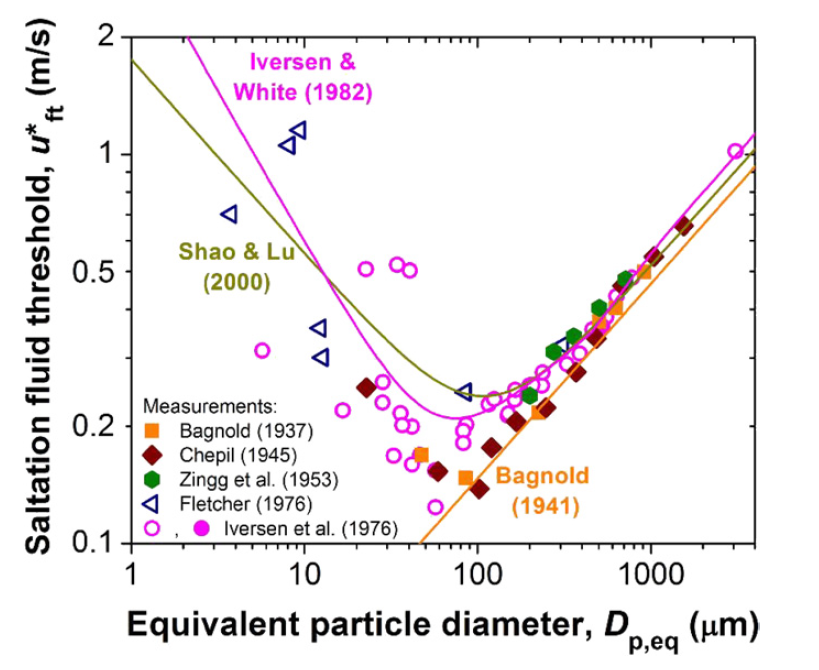
\includegraphics[scale=0.7]{../figs/Threshold_friction_velocity.PNG}
    \caption{Threshold friction velocity $\mathbf{u^*}$ as a function of particle diameter. Points represent measurements from wind tunnel experiments, and the lines represent different semi-empirical expressions for the threshold friction velocity \parencite{kok2012physics}}.
    \label{fig:treshold_friction_velocity_ps}
\end{figure}}  
All these factors vary significantly both spatially and temporally, making accurately calculating the threshold friction velocity difficult \todo{reference}. \Cref{fig:treshold_friction_velocity_ps} show the the threshold friction velocity as a function of particle diameter, the coloured lines represent the semi-empirical relations for $u^*_t$ described in \textcite{iversen1982saltation} (pink), \textcite{shao2000simple} (green) and \textcite{bagnold1941physics}.
The semi-empirical relations and measurement seems to agree on a minimum in $u^*_t$ around in the range between  \SI{75}{\micro\metre} - \SI{100}{\micro\metre}.
However, these particles are too heavy to be subject to long-range suspension in the air and will soon after entrainment take on ballistic trajectories.
The process of the wind transporting large dust particles through a series of "jumps" across the surface is called saltation. 
The impact from the large particle hitting the soil bed ejects smaller dust particles (\SI{20}{\micro\metre} < ) and 
these smaller particles can be subjected to long-range transport. This process, known as sandblasting, is the predominant process causing dust emissions \parencite{kok2012physics}. The direct dust entrainment processes are often minor compared to sandblasting and, therefore, often neglected in dust models.

Several physics-based schemes for estimating the vertical dust emission according to the saltation theory have been proposed \parencite{MB95_dust_emission,alfaro2001modeling,shao2004simplification}. 
The main distinction between the present schemes lies in how the particle size information is represented. The schemes can be divided into one of two categories, bulk and size resolving dust emission schemes.
The bulk schemes (e.g. the emission scheme by \parencite{MB95_dust_emission}) gives an estimate of the total dust flux, $F$ but provide no information about particle size-resolved dust flux $F(d)$. The bulk dust flux is estimated by first calculating the horizontal saltation flux (i.e. how many large particles there are jumping along the surface) and then deriving the vertical flux from the horizontal dust flux \parencite{tegen2014numerical}.
The scheme of \textcite{MB95_dust_emission} uses an empirical relation to relate saltation to the bulk dust vertical flux by scaling the saltation flux by a proportionally constant that depends on the clay content of the soil. In bulk emissions schemes, the vertical dust flux $F(d)$ of different particle sizes is inferred by assuming a fixed size distribution of the emitted dust particles $p_s(d)$ due to saltation.
Based on the theory of brittle fragments \textcite{kok_scaling_2011} derived theoretical expression of the particle size distribution for dust particles between \SI{0.1}{\micro\metre} - \SI{20}{\micro\metre} which showed good agreement when compared against observed size distributions of emitted dust. 
The \textcite{kok_scaling_2011} size distribution has been included in most dust models and has been shown to improve the representation of dust aerosols when compared to observations \parencite{johnson2012global}.
However, this particle size distribution only applies to dust emission events that are predominantly due to the fragmentation of soil aggregates \parencite{kok2012physics}.

% \begin{equation}\label{eq:shao04}
%     F(d_i;d_s)=c_y\eta \left[(1-\gamma)+\sigma_p\right](1+\sigma_m)\frac{Q(d_s)g}{u_*^2}
% \end{equation}

The particle size resolving schemes, e.g. \textcite{shao2004simplification}, can directly derive the size-resolved dust flux $F(d_i)$. This scheme calculates the emissions of particles with a size $d_i$ generated by saltating particles of size $d_s$. However, these schemes require knowing the parent soil particle size distribution, and measurements of parent soil particle size distributions are not available on a global scale.

Lastly, the surface roughness $z_0$ is an important parameter for calculating the friction velocity required for estimating the dust emissions. The $z_0$ used in global and regional models contain information about the subgrid-scale topography and vegetation to reproduce realistic grid-scale winds. However, these roughnesses operate on different spatial scales than the physical processes involved in dust emissions, which can introduce biases in the estimated dust flux \parencite{darmenova_development_2009}. Therefore some models employ a satellite-derived dataset of surface roughness to obtain roughness on scales relevant for aeolian processes. 


\subsection{Dust transport}
Dust transport is divided into several different regimes as illustrated in \Cref{fig:modes_of_dust_transport}, which mode of transport a dust particle is subjected to is predominately determined by the local wind speed and the size of the particle. Among the different modes of transport, only long term suspension is usually considered in current dust models.
While dust particles with the longest lifetime in the atmosphere are less than \SI{20}{\micro\metre}, there is a growing amount of evidence that under the right atmospheric conditions, even giant dust particles larger than \SI{200}{\micro\metre} can be transported for thousands of kilometres \parencite{van2018mysterious}. 
In comparison with observation, current dust models struggle with representing the coarse particle, i.e., severely underestimating the lifetime of the coarse dust particles while overestimating the fine mode \parencite{adebiyi2020dust}. 
\begin{figure}[htbp]
  \centering
  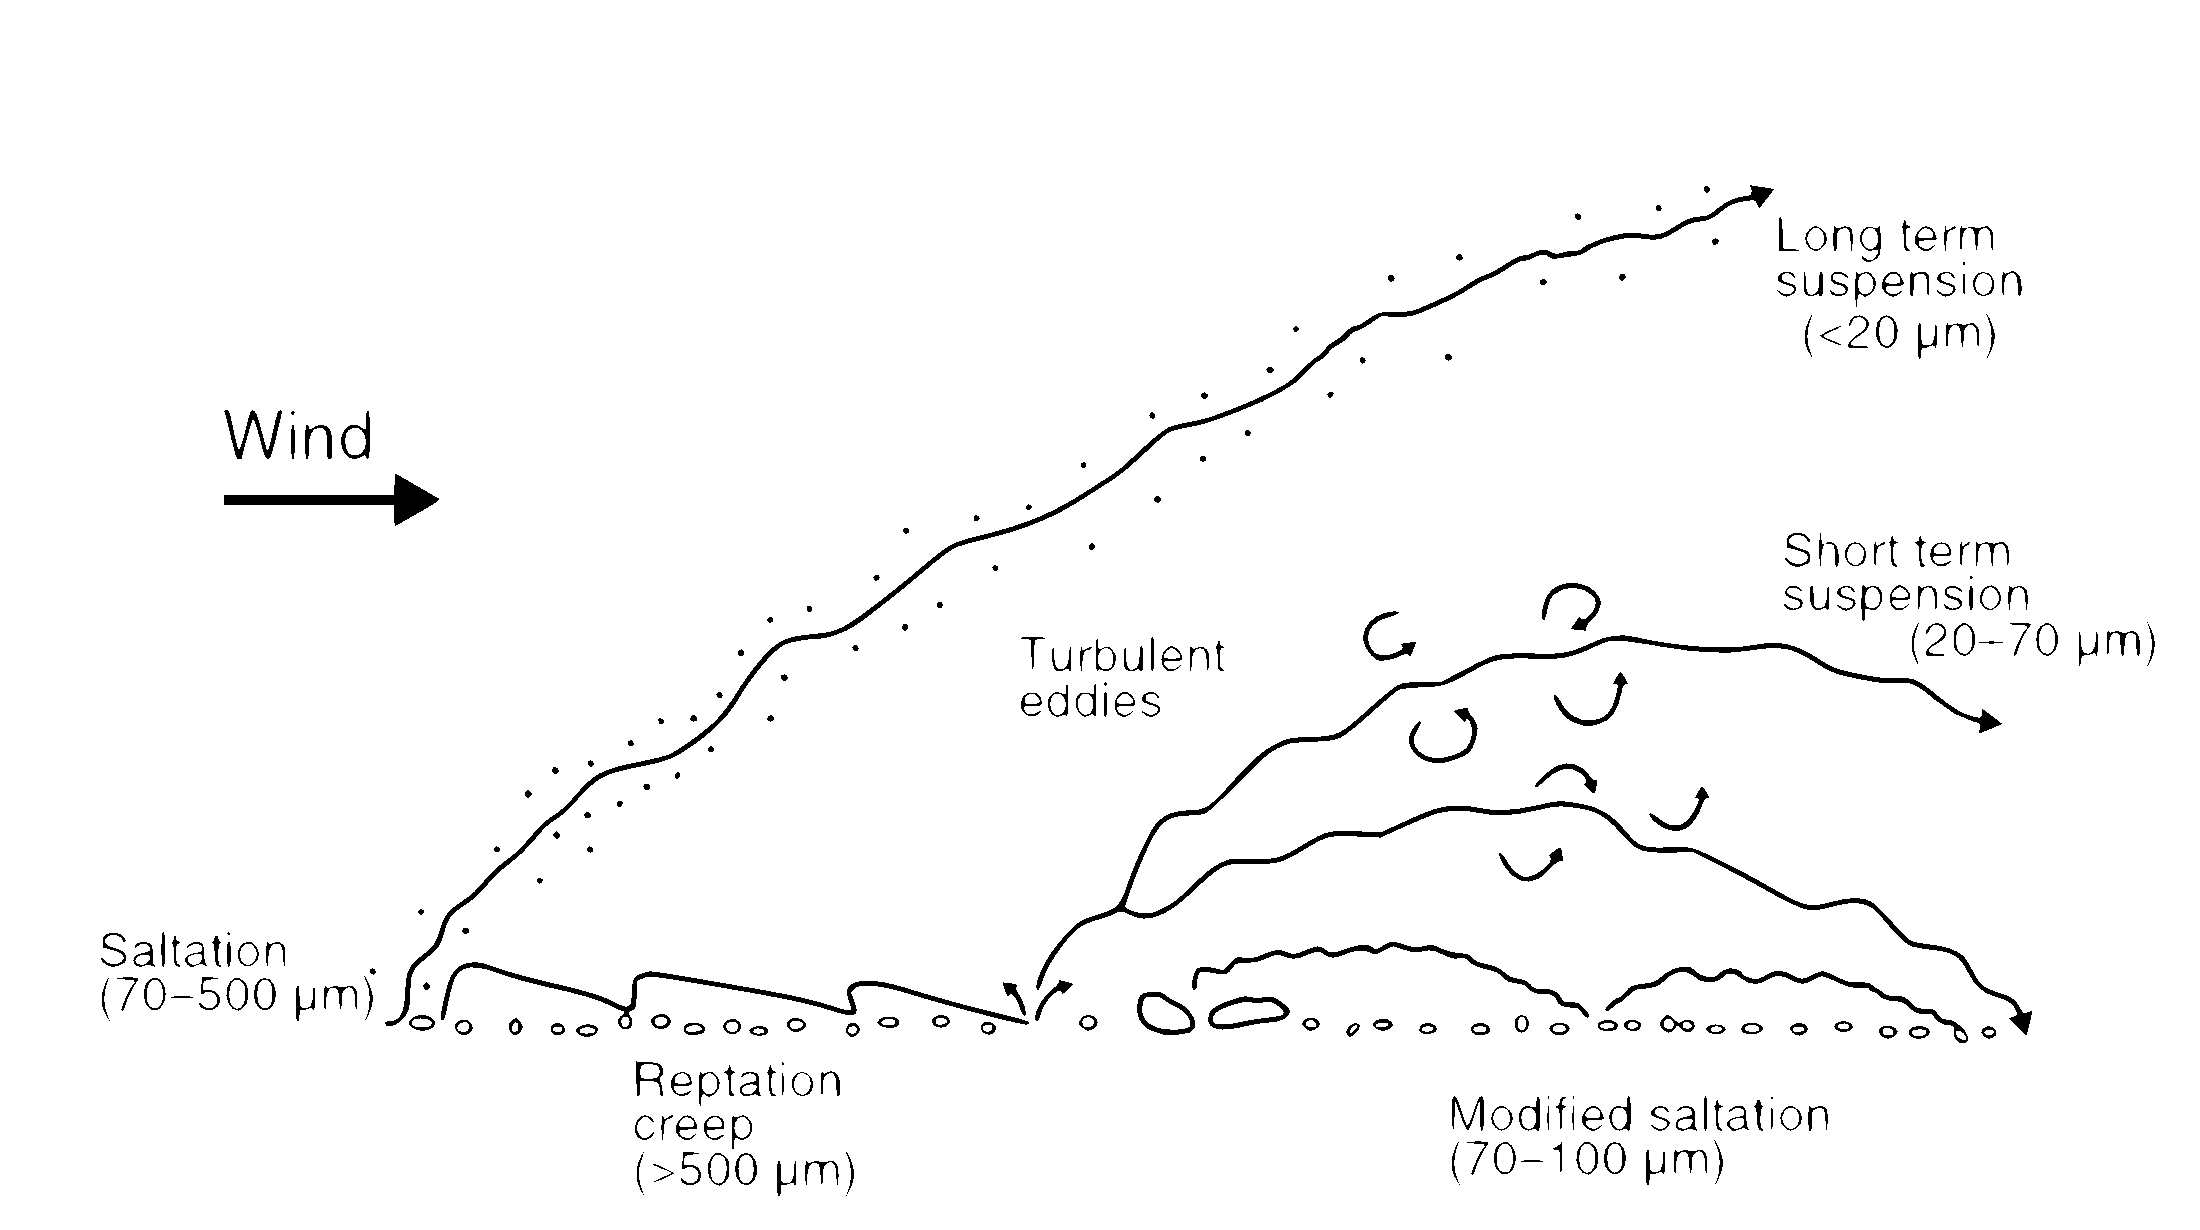
\includegraphics[draft=false,width = \textwidth]{texfiles/figs/aeolian_transport_Parsons_Abrahams.pdf}
  \caption{Different regimes of aeolian transport \parencite{nickling2009aeolian}}
  \label{fig:modes_of_dust_transport}
\end{figure}

Part of the reason why coarse dust is not well represented in current dust models is that they typically are non-spherical. Non-sphericity can have a significant impact on the settling velocity of the particle due to increased aerodynamic drag. The effect of the non-sphericity on settling velocity of dust particles was investigated by \textcite{mallios2020effects}, and they found that non-spherical dust particles could remain significantly longer in the atmosphere compared to spherical particles of equivalent particle diameter. The non-sphericity of dust particles is not included in most dust models \parencite{huang2020climate}. Moreover, dust models cannot directly model the turbulent properties of the near-surface flow. The surface turbulence is important for the entrainment of coarse dust \parencite{klose2013large} and in facilitating the dust to stay aloft longer \parencite{ryder2013impact}. Electric charging of the dust particles counteracting the gravitational settling has also been proposed to affect the lifetime of large dust particles and remains to be explored in dust models. Lastly, \textcite{heisel2021gentle} suggested that gentle sloping topography increased the chance for the coarse particles to reach higher altitudes.  

The transport of atmospheric dust can either be simulated in a Lagrangian or Eulerian framework.
In the Lagrangian framework, the dust is treated as a discrete entity represented by many computational particles.
The computational particles are suspended with the flow, and their trajectories are determined by integrating the particle motion. 
The dust concentration rarely exceeds more than several grams per kilogram of air. Therefore, the presence of dust aerosols does not significantly impact the density and dynamics of the flow \parencite{zhuang2001compositions}. Consequently, the motion of the dust particles can be determined separately from fluid motion \parencite{ShaoYaping2008PaMo}.
Lagrangian models rely on tracking many computational particles to obtain statistically robust results and can thus be computationally expensive. 

In eulerian models implemented in most climate and weather forecast models, the dust aerosols are assumed to behave like a fluid. Therefore, the dust concentration follows the same kind of advection and conservation equations as other scalars in the atmosphere. 
In an Eulerian dust model, the atmosphere is discretised into grid boxes on a computational grid with a certain resolution, and in each grid box, the model calculates the dust concentration. However, because of the limited resolution of the grid, Eulerian models often suffer from excessive numerical diffusion, which causes filament structure in the transport to be smoothed out \parencite{cassiani_offline_2016}. 
In contrast, Lagrangian models do not require a computational grid and can therefore better preserve such filament structures in the transport \parencite{cassiani_offline_2016}.         

\subsection{Dust deposition}
Dust can be removed from the atmosphere either through dry- or wet deposition. 
Dry deposition typically is the dominant process close to the source region as there are still many large dust particles present that falls out quickly. 
As the dust is transported further away from the source region, the larger particles fall out, and the dust size spectrum becomes narrower and the mode finer \parencite{does2016particle}.
Dry deposition becomes less efficient at finer particle sizes, and thus far from the source, wet deposition is usually the dominating process \parencite{zhao2003modeled}.


In dust models, the deposition is typically represented by a deposition velocity. 
The predominant factors deciding the deposition velocity for dry deposition are the dust particle size and the density. A multi-layer resistance scheme is commonly used in dust models to estimate the dry deposition rate. A widely used scheme used for modelling dry deposition is the two-layer resistance model of \parencite{slinn1982predictions}. 
The resistance model divides the atmosphere into two distinct layers; The quasi-laminar sublayer close to the ground, which has a thickness on the order of centimetres and the constant flux layer above. In the quasi-laminar sublayer, Brownian diffusion and gravitational settling are the two main deposition processes. Within the constant flux layer, turbulent motions and gravitational settling dominate. The gravitational settling velocity can be expressed by the modified stokes law of \parencite{slinn1982predictions}: 
\begin{equation}
    v_g = \frac{g\rho_p d_p^2 C_{cun}}{18\mu}
\end{equation}
Where $\rho_p$ and $d_p$ is the particle density and diameter, $\mu$ is the dynamic viscosity of air and $C_{cun}$ is the Cunningham slip-flow correction. The slip-flow correction accounts for the reduction in the drag force experienced by the smallest particles of sizes comparable to the mean free path of the molecules in air. The dry deposition velocity of a particle with a given size is given by a set of resistances, added to the settling velocity $v_g$:
\begin{equation}\label{eq:drydep_resistance}
    v_d=[r_a + r_b + r_a r_b v_g]^{-1} + v_g
\end{equation}
Here the $r_a$ represent the aerodynamic resistance in operating the constant flux layer, and $r_b$ represent the resistance in the quasi-laminar surface layer. 
There have been relatively few theoretical developments since the work of \textcite{slinn1982predictions} even though this model has been shown to reproduce the dependence of $v_d$ on particle size, it does not differentiate the deposition velocity between different surfaces \parencite{shao2011dust}.
The difference in deposition rate between different surfaces is expected to be quite large \parencite{bergametti2018size,zeng2019deposition}. 

There are two distinct routes for wet deposition: a dust particle can be wet deposited, in-cloud or below-cloud scavenging: 
In-cloud scavenging, the dust particles are rained out from the cloud through serving as \acrshort{ccn}s or \acrshort{in}s or by colliding with existing cloud particles. Below-cloud scavenging involves the dust particles being captured by falling hydrometeors. 
Many of the mechanisms involved in wet deposition are complex and generally not well understood,\todo{citation} and some dust models do not consider wet deposition at all \parencite{zhang2019parameterization}. Between below-cloud and in-cloud scavenging, below-cloud scavenging is the simpler and better-studied process.
Two mechanisms have been suggested to affect the efficiency of below-cloud scavenging: (1) fine dust particles with diameters less than \SI{2}{\micro\metre} tend to follow the streamlines and flow around the droplet, and (2) the dust particles might bounce off after colliding with the droplet. 
Accordingly, below-cloud scavenging is typically most efficient for the larger dust particles \parencite{jung2006intercomparison}.
Currently, data is lacking for determining the probability of retention during the collision with the droplet, hence this mechanism is not included in current dust deposition schemes \parencite{ShaoYaping2008PaMo}. Several schemes for estimating the below-cloud scavenging efficiency $\lambda$ of varying levels of complexity have been proposed. 
The more advanced schemes, e.g. \textcite{seinfeld1998atmospheric, ShaoYaping2008PaMo}, uses semi-empirical relations to explicitly calculate the collection efficiency $E(r,R)$ as a function of both the droplet and dust particle radius.
However, these schemes require knowing droplet size distribution which is not always available in the model. 
Therefore empirical below cloud scavenging schemes that directly relate scavenging coefficient to the precipitation rate, e.g. \textcite{brandt2002modelling} have been developed. 
These schemes avoid uncertainties in determining the collection efficiency \parencite{jung2006intercomparison}. 
Some empirical schemes, e.g. \textcite{laakso2003ultrafine} also includes a dependence of dust particle size for the scavenging efficiency. 
\begin{figure}[htpb]
    \centering
    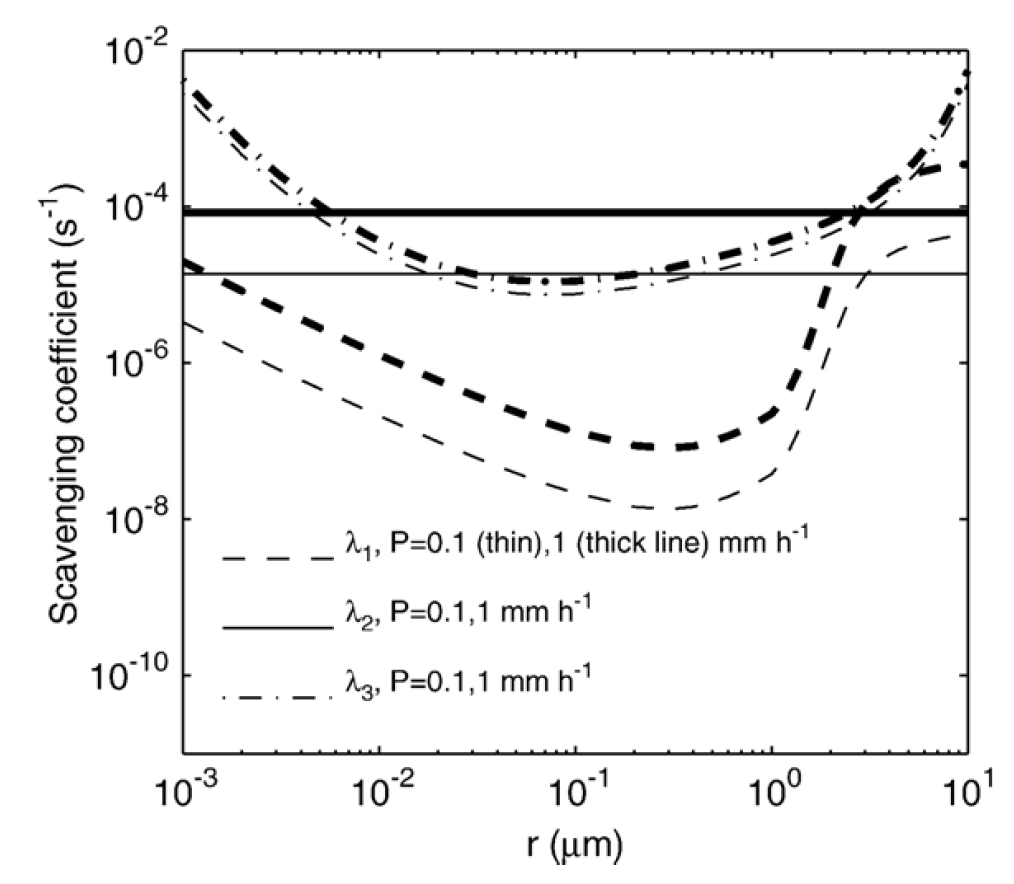
\includegraphics[draft=False,scale=.5]{texfiles/figs/Scavenging.PNG}
    \caption{Comparison of below cloud scavenging coefficients for three different below-cloud scavenging schemes; $\lambda_1$ \textcite{jung2006intercomparison},$\lambda_2$ \textcite{brandt2002modelling} and $\lambda_3$ \textcite{laakso2003ultrafine}. 
    P is the precipitation rate (units: \si{\mm\per\hour}) 
    Adopted from \textcite{jung2006intercomparison}}.
    \label{fig:scavenging}
\end{figure}
A comparison of the semi-empirical \textcite{ShaoYaping2008PaMo} scheme and empirical \textcite{brandt2002modelling} and \textcite{laakso2003ultrafine} are shown in \Cref{fig:scavenging}. For all the schemes, $\lambda$ increases for larger precipitation rates. Moreover, in the two schemes where $\lambda$ depends on the size of the dust particle, the scavenging coefficient decreases towards the \SI{1}{\micro\metre} mark and then increase again for the dust particles larger than \SI{2}{\micro\metre}. 

Present understanding of in-cloud processing and especially for dust aerosols, is lacking. 
Thus the representation of in-cloud removal of dust in models remains crude. Some dust models represent the dust as purely hydrophobic and neglect in-cloud scavenging entirely, while other models assume dust scavenging efficiency to be that of sulphate \parencite{bergametti2014dust}. 
Yet deposition is a key aspect of the dust cycle and cannot be represented without an adequate representation of the wet removal process.
